%% LaTeX Beamer presentation template (requires beamer package)
%% see http://bitbucket.org/rivanvx/beamer/wiki/Home
%% idea contributed by H. Turgut Uyar
%% template based on a template by Till Tantau
%% this template is still evolving - it might differ in future releases!

\documentclass[mathserif,profesionalfont,10pt,dvips,xcolor=table]{beamer}

\mode<presentation>
{
\usetheme{Warsaw}
\usecolortheme{wolverine}

\setbeamercovered{transparent}
}

\usepackage[utf8x]{inputenc}
\setbeamersize{text margin left=.5cm, text margin right=.5cm}

%\usepackage[scaled=.8]{ae}
% font definitions, try \usepackage{ae} instead of the following
% three lines if you don't like this look
%\usepackage{mathptmx}
\usepackage[scaled=.90]{helvet}
%\usepackage{courier}
\usepackage[T1]{fontenc}
% hyperlinks
\hypersetup{colorlinks}
\usepackage[colorlinks=true]{hyperref}
\hypersetup{pdfautor={Alfredo S\'anchez Alberca (asalber@ceu.es)}, pdftitle={rkTeaching: un paquete para la ense\~{n}anza de Estad\'{\i}stica con R}}
\usepackage[spanish]{babel}

\setlength{\parskip}{0.5em}

\newcommand{\glad}{
\includegraphics[scale=0.06]{img/glad-icon}}
\newcommand{\sad}{
\includegraphics[scale=0.06]{img/cry-icon}}

\theoremstyle{definition}
\newtheorem{objetive}[theorem]{\translation{Objetivo}}

\title{\textbf{rkTeaching}:\\ Un paquete de R para la enseñanza de Estadística}

\author[Alfredo Sánchez Alberca]{Alfredo Sánchez Alberca\\ (\texttt{asalber@ceu.es})}

\institute[Universidad San Pablo CEU] {
Departamento de Matemáticas\\ 
Universidad San Pablo CEU\\[1cm]

\includegraphics[scale=0.2]{img/logo_jidere}
}

\date{16 de julio de 2012}


% This is only inserted into the PDF information catalog. Can be left
% out.
\subject{Talks}

\begin{document}

\begin{frame}
\titlepage
\end{frame}

\begin{frame}
\frametitle{Contenidos}
\tableofcontents[hideallsubsections]
% You might wish to add the option [pausesections]
\end{frame}


\section{Introducción}

\subsection{La enseñanza de Estadística en la USP CEU}
\begin{frame}
\frametitle{La enseñanza de Estadística en la USP CEU}
La estadística es una materia básica en las ciencias de la salud. En la USP CEU se imparte en  
\begin{itemize}
\item Medicina
\item Farmacia
\item Psicología
\item Fisioterapia
\item Enfermería
\item Óptica
\item Nutrición 
\end{itemize}
\end{frame}


\subsection{Software para el tratamiento de datos}
%-----------------------------------------------------------------------------------------------------slide--------------
\begin{frame}
\frametitle{Software para el tratamiento de datos}
En la última década se han utilizado distintas aplicaciones para el tratamiento de datos en los análisis estadísticos:
\begin{description}
\item[Excel]
\begin{itemize}
\item[\glad] Muy conocida y extendida
\item[\glad] Fácil de usar para análisis sencillos
\item[\sad] No incorpora procedimientos para análisis más complejos
\end{itemize}
\item[Statgraphics]
\begin{itemize}
\item[\glad] Bastante pedagógica (dificultad de aprendizaje: baja-media)
\item[\sad] Muy extendida en el ámbito universitario pero poco en el hospitalario
\end{itemize}
\item[SPSS] 
\begin{itemize}
\item[\glad] Muy extendida en el ámbito hospitalario
\item[\glad] Poco pedagógica (dificultad de aprendizaje: media-alta)
\item[\sad] Muy potente (incorpora su propio lenguaje de programación)
\end{itemize}
\end{description}
Sin embargo, todas ellas comparten serios inconvenientes: 
\begin{itemize}
\item[\sad] \alert{No son aplicaciones libres}
\item[\sad] \alert{No son fácilmente adaptables a las necesidades docentes}
\end{itemize} 
\end{frame}


\section{Introducción de R}
%-----------------------------------------------------------------------------------------------------slide--------------
\subsection{R: La apuesta por el Software libre}
\begin{frame}
\frametitle{R: La apuesta por el Software libre}
Desde 2008, el Departamento de Matemáticas de la USP CEU ha hecho una apuesta fuerte por el uso del software libre en la enseñanza de la Estadística.

La elección más lógica fue el programa R (\url{http://www.r-project.org/}):
\begin{itemize}
\item[\glad] Es software libre
\item[\glad] Es multiplataforma (Unix/Linux, Windows, Mac)
\item[\glad] Mantenido por una enorme comunidad de desarrolladores en todo el mundo
\item[\glad] Tiene su propio lenguaje de programación
\item[\glad] Tan potente como SPSS (o más)
\end{itemize}
Pero 
\begin{itemize}
\item[\sad] Dificultad de aprendizaje alta
\item[\sad] No disponde de interfaces gráficas de usuario (GUI) amigables
\end{itemize}
\begin{objetive}
Desarrollar una interfaz de usuario sencilla para facilitar la enseñanza de la Estadística y reducir la curva de aprendizaje de R.
\end{objetive}
\end{frame}


\subsection{Interfaz gráfica de usuario de R}
%-----------------------------------------------------------------------------------------------------slide--------------
\begin{frame}
\frametitle{Elección de la interfaz gráfica de usuario R Commander}
Actualmente existen varias interfaces gráficas de usuario para R (\url{http://www.sciviews.org/_rgui/}), pero la mayoría están pensadas para usuarios avanzados o programadores de R.

En 2008 se optó por R Commander (John Fox 2005):
\begin{itemize}
\item[\glad] Orientada a usuarios no expertos
\item[\glad] Multiplataforma
\item[\glad] Ampliable mediante un sistema de plugins
\item[\sad] Basada en librerías gráficas Tcl/Tk (bastante anticuadas)
\item[\sad] Salida en texto plano bastante pobre 
\end{itemize}
Se desarrolló el paquete RcmdrPluginTeachingExtras que se utilizó durante dos años para impartir las prácticas de Estadística.
\end{frame}


\subsection{Migración a RKWard}
%-----------------------------------------------------------------------------------------------------slide--------------
\begin{frame}
\frametitle{Migración a RKWard}
En 2010 se lanza la versión 0.5.5 RKWard (Thomas Friedrichsmeier 2002):
\begin{itemize}
\item[\glad] Orientada a todo tipo de usuarios, tanto expertos como no expertos
\item[\glad] Multiplataforma
\item[\glad] Fácilmente ampliable mediante un sistema de plugins
\item[\glad] Basada en librerías gráficas Qt (mucho más modernas)
\item[\glad] Salida en formato html
\end{itemize}
Se decide migrar el plugin de R Commander a esta nueva interfaz de usuario.
\begin{center}

\includegraphics[scale=0.5]{img/logo_rkward}
\end{center}
\end{frame}


\section{Desarrollo de rkTeaching}
%-----------------------------------------------------------------------------------------------------slide--------------
\begin{frame}
\frametitle{Desarrollo de rkTeaching}
Sobre la base de RKWard se ha desarrollado el plugin rkTeaching.
 
Ha sido concebido para facilitar el aprendizaje de Estadística:
\begin{itemize}
\item Simplicidad (eliminación de las opciones más complejas)
\item Adaptado a la programación de la enseñanza la Estadística en la USP CEU
\item Asistente de ayuda al usuario
\item Salidas orientadas a facilitar la comprensión del alumno/a
\end{itemize}
\end{frame}


\section{Comparativa docente de rkTeaching vs SPSS}
%-----------------------------------------------------------------------------------------------------slide--------------
\begin{frame}
\frametitle{Comparativa docente de rkTeaching vs SPSS }
Se realizó un estudio comparativo de la facilidad de uso y el tiempo de aprendizaje entre rkTeaching y SPSS.

Se tomó una muestra de 40 alumnos de medicina que habían hecho el curso básico de estadística pero nunca habían manejado rkTeaching ni SPSS.

Cada alumno tuvo que realizar una serie de ejercicios (introducción de datos, dibujo de histograma, cálculo de estadísticos descriptivos, cálculo de modelo de regresión lineal, cálculo de probabilidad normal y test t para la comparación de medias) con cada programa y al final se les pasó una encuesta sobre la facilidad de uso.

Variables medidas:
\begin{itemize}
\item \texttt{TiempoR}:Tiempo de realización de la tarea con rkTeaching (en min).
\item \texttt{TiempoSPSS}: Tiempo de realización de la tarea con SPSS (en min).
\item \texttt{FacilidadR}: Facilidad de uso de rkTeaching (escala discreta de 1=más difícil a 5=más fácil).
\item \texttt{FacilidadSPSS}: Facilidad de uso de SPSS (escala discreta de 1=más difícil a 5=más fácil).
\end{itemize} 
\end{frame}


%-----------------------------------------------------------------------------------------------------slide--------------
\subsection{Comparativa de tiempo de aprendizaje}
\begin{frame}
\frametitle{Comparativa del tiempo de aprendizaje de rkTeaching vs SPSS}
\begin{columns}
\begin{column}{0.5\textwidth}
\begin{center}
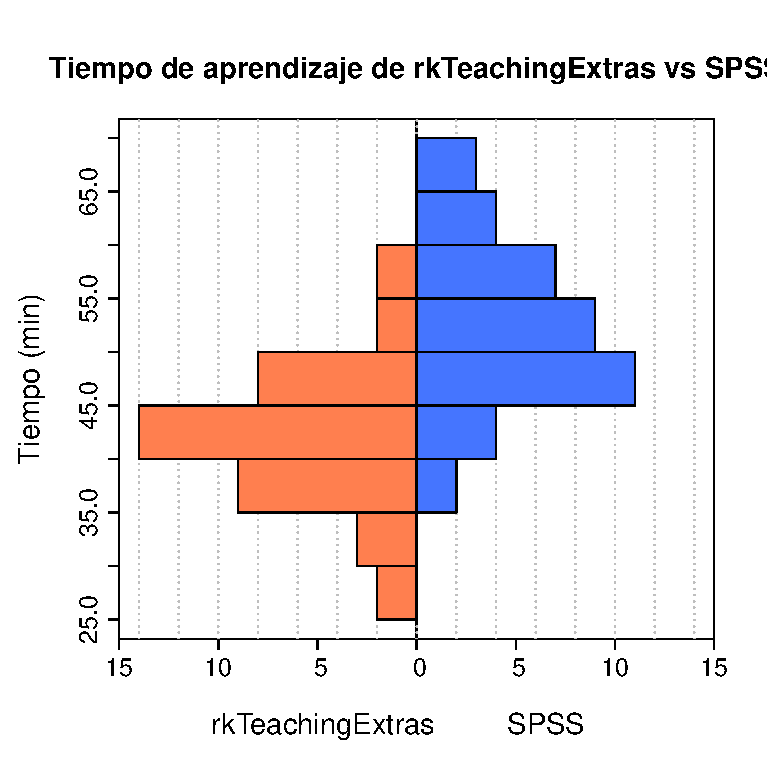
\includegraphics[scale=0.5]{img/histograma_aprendizaje}
\end{center}
\end{column}
\begin{column}{0.45\textwidth}
El tiempo de aprendizaje de SPSS fue significativamente mayor que el tiempo de aprendizaje de rkTeaching:
\begin{itemize}
\item p-valor: $4.8e-17$
\item Intervalo de confianza del 95\% para diferencia de medias: $(9.06,\, \infty)$
\end{itemize}
El tiempo medio para realizar las tareas con SPSS fue al menos 9 minutos mayor que el de rkTeaching, lo que supone una reducción del tiempo de al menos un 17\%.
\end{column}
\end{columns}
\end{frame}



%-----------------------------------------------------------------------------------------------------slide--------------
\subsection{Comparativa de facilidad de uso}
\begin{frame}
\frametitle{Comparativa de facilidad de uso de rkTeaching vs SPSS}
\begin{columns}
\begin{column}{0.5\textwidth}
\begin{center}
\includegraphics[scale=0.35]{img/barras_facilidad}
\end{center}
\end{column}
\begin{column}{0.45\textwidth}
La facilidad de uso rkTeaching fue significativamente mayor que la de SPSS:
\begin{itemize}
\item p-valor: $1.7e-06 $
\item Intervalo de confianza del 95\% para diferencia de medias: $(0.4993,\, \infty)$
\end{itemize}
La facilidad de manejo de rkTeaching es de al menos medio punto más que con SPSS, lo que supone un aumento de la facilidad de al menos un 10\%. 
\end{column}
\end{columns}
\end{frame}


%-----------------------------------------------------------------------------------------------------slide--------------

\section{Conclusiones}

\begin{frame}
\frametitle<presentation>{Conclusiones}
\begin{itemize}
\item RKWard es una interfaz gráfica de usuario fácilmente ampliable y adaptable a través de plugins.
\item Se ha desarrollado el plugin rkTeaching para facilitar la enseñanza de la Estadística.
\item Se ha elaborado un libro de prácticas con rkTeaching.
\item rkTeaching se ha utilizado para impartir las prácticas de Estadística en las titulaciones de Ciencias de la Salud de la USP CEU con éxito. 
\item El aprendizaje de rkTeaching por parte de los alumn/as es más rápido que el de SPSS.
\item rkTeaching es más fácil de usar que SPSS por parte de los alumno/as.   
\end{itemize}
\end{frame}

%-----------------------------------------------------------------------------------------------------slide--------------
\begin{frame}
\frametitle{Trabajo futuro}
\begin{itemize}
\item Traducción de rkTeaching al castellano. 
\item Mejorar la salida con interpretaciones de los resultados. 
\item Incorporar cuadros de diálogo para análisis más complejos (análsis multivariante).
\end{itemize}
\end{frame}

\end{document}
